\documentclass{report}
\usepackage{titlesec}
\usepackage{float}
\usepackage{rotating}

\titleformat{\chapter}[block]{\LARGE \bfseries}{Chapter \arabic{chapter}}{1em}{}[]
\title{ DJI M300 platform development plan}
\author{Shun Li, Zhewen Xing, Linhan Qiao }
\date{\today}

\begin{document}
\maketitle
\tableofcontents

\chapter{Objects}
From easy to hard, currently a 4-steps development plan is proposed after our
discussion, which is shown below in the form of 4 list following by several
sub-tasks.

\section{Communication:}

In this step, we aim to get familiar with the whole platform, establish
the connection between the onboard computer, sensors as well as the
drone autopilot.
\\
Only the \textbf{ground test} is needed to achieve this step.
\\
\\
\textbf{Sub-Tasks:}

\begin{itemize}
    \item Read the state estimation data( height, velocity, acceleration,
        attitude, latitude, longitude, etc.)
    \item Send the test command to the camera and autopilot, check the
        responding.
    \item Read, store and covert the RGB and IR images 
\end{itemize}


\section{Waypoint flight}

In this step, the automatically flight along the given path should be
conducted. The onboard computer can control the drones to fly along a
given path, and take photos at some certain waypoint.
\\
Both \textbf{ground test} and \textbf{flying test }are needed in this step.
\\
If the synthetic fire and smoke can be done outdoor, we could make a
data set by combining the RGB and IR images captured by the drone and
H20T.
\\
\\
\textbf{Sub-Tasks:}
\begin{itemize}
    \item Waypoint flight simulation with simulator provided by
        DJI.
    \item Accomplish some given mission( take a photo, drop something,
        etc.) at a certain waypoint
    \item Fly along the given path(waypoints) and take the picture(RGB
        and IR) of the synthetic fire and smoke(an oven, if possible) 
\end{itemize}


\section{Fire and smoke detection:}
In this step, The forest fire detector should run on the YunGuan2.0 onboard
computer, detect and segment the fire and smoke in real time while the drone
flies along the given path.
\\
Please note that there is no feedback from the detector to the navigation part
for the path replanning, the 2 parts work separately.
\\
Both the ground and flying test are needed in this step.

\begin{itemize}
    \item Implement the fire and smoke detector which runs on the 
        onboard computer.
    \item DJI M300 flies along the path and detects the synthetic fire
        and smoke along the path
\end{itemize}

\section{Detection and Navigation}

In this step, the feedback from the detector is established for the path
planning and replanning after the fire or smoke is detected.
\\
Also, both the ground and flying test are needed in this step.

\begin{itemize}
    \item Detect fire and  Navigate around the fire according to some 
        given strategy
    \item Motion control under the navigation module after the fire is 
        detected.
\end{itemize}


\chapter{Schedule}

According to the annual climate data, the temperature will be only around 10 °C
by the end of October.
\begin{figure}[H]
    \centering
    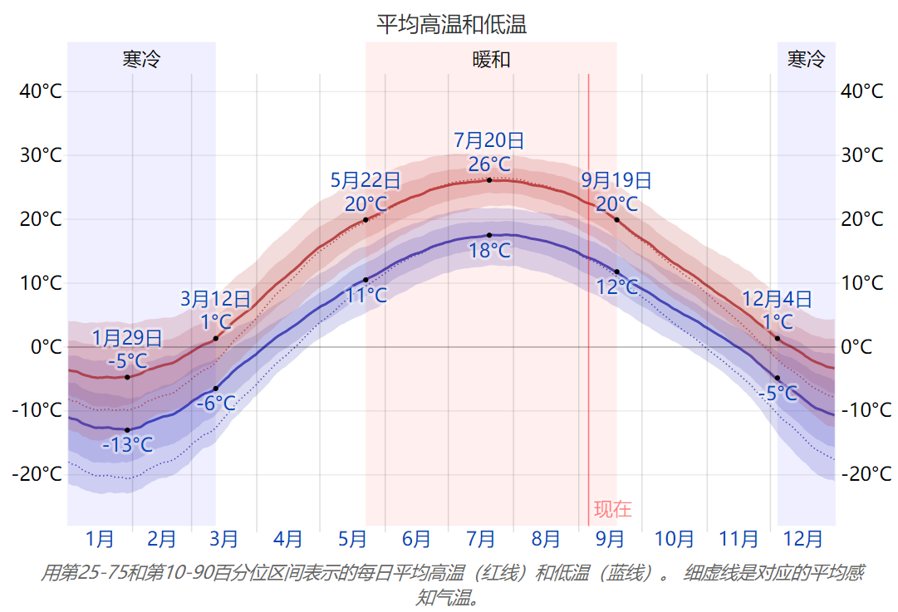
\includegraphics[width=1\textwidth]{climate}
    \caption{The annual temperature of Montreal}
\end{figure}

Once it is lower 10 °C outdoors, it will be harmful for the battery working and also
very cold for us to perform the experiment. So the following timetable is ended
by the end of October, 2021.

The hight rows stand for the 2 outdoors experiment content and time.

\begin{sidewaystable}
    \begin{figure}[H]
        \centering
        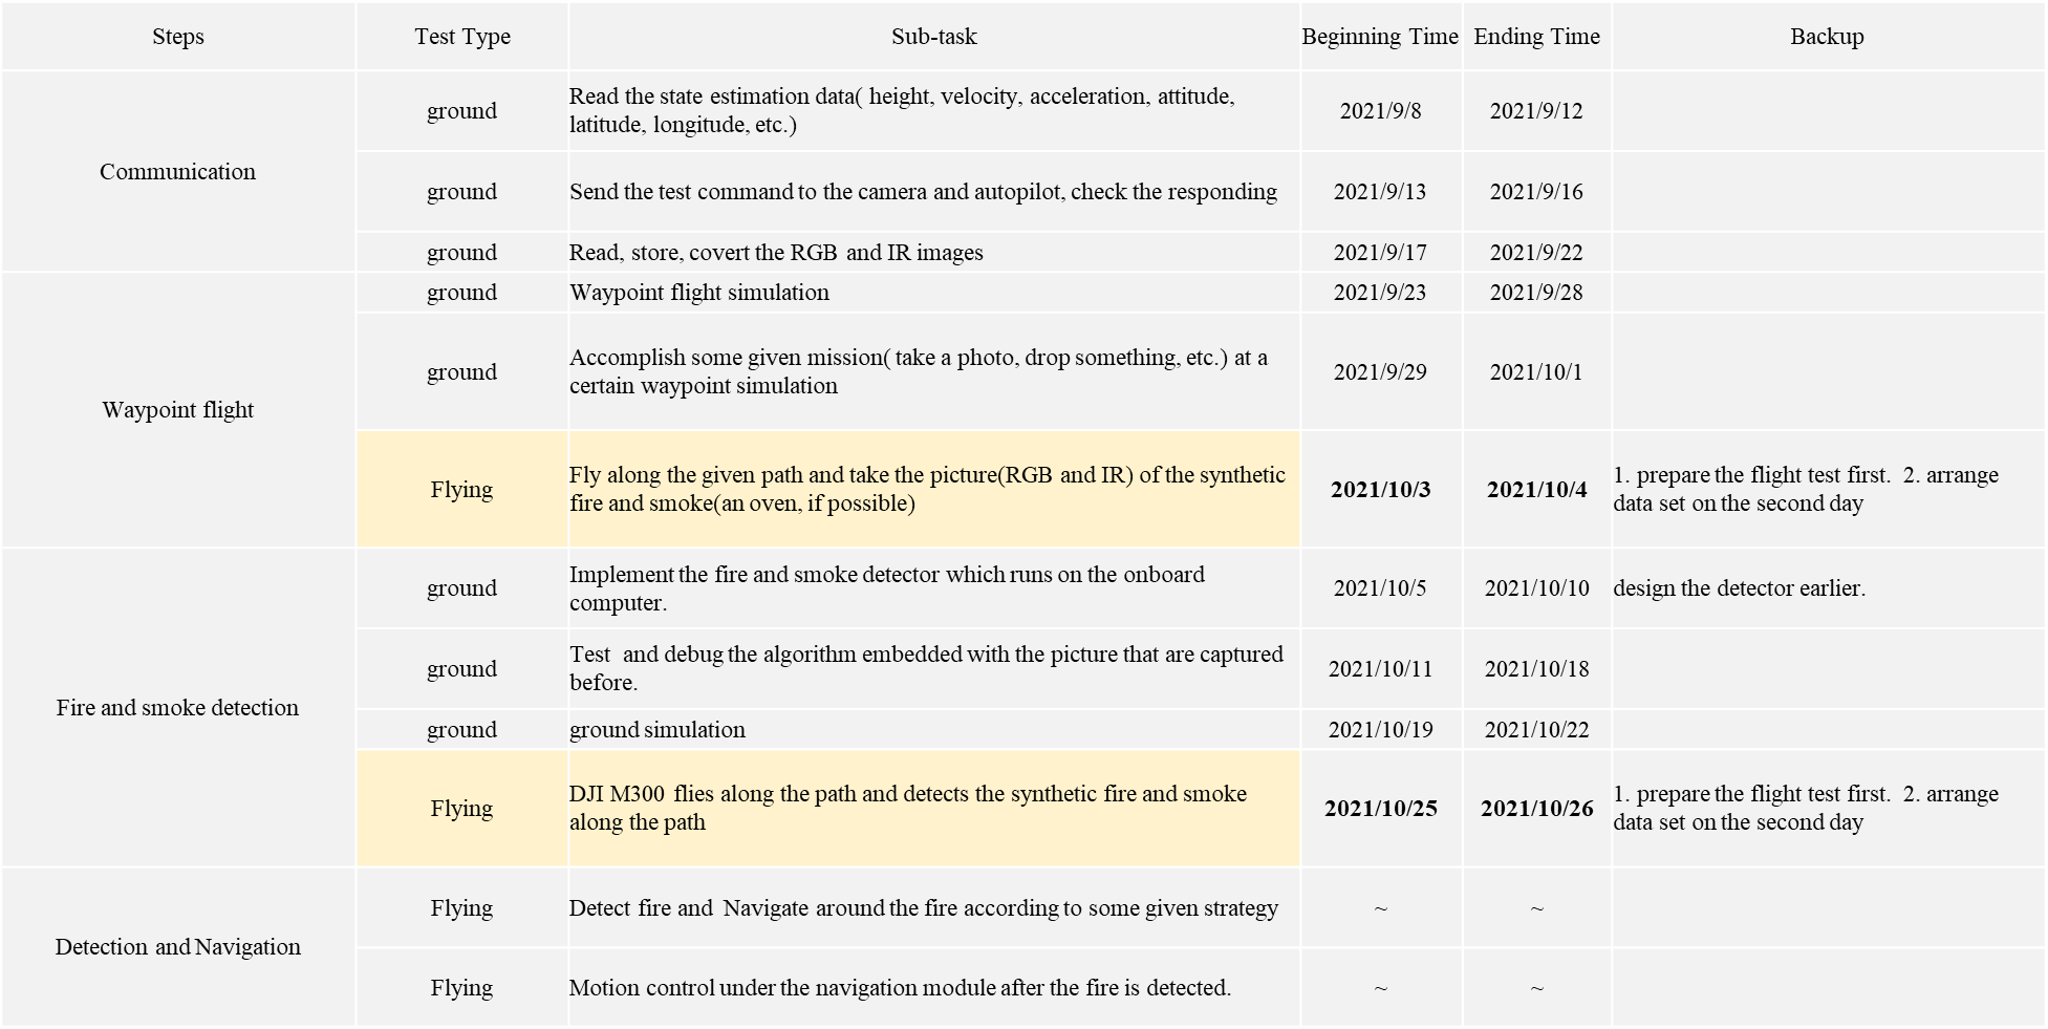
\includegraphics[width=1.2\textheight]{timetable}
    \end{figure}
    \caption{Timetable}
    \label{fig_timetable}
\end{sidewaystable}


\chapter{Challenges}
 In this section, some of the currently known challenges to use the platform are
 demonstrated below:

\section{Transplantation of the Algorithm }
Although we currently have the mature detection algorithm, the transplantation
to the onboard computer may be an onerous task. It may involve some knowledge of
the software engineering and embedding system.

\section{Monitoring and Display the real-time experiment}
We may want to monitor the self-developed detector and navigation algorithm
while in the real-time experiment. To accomplish that, we need to pass back the
images both captured by the H20T and after the detection with mask, as well as
the path planned by the navigation module. So the passing back could be a hard
task to accomplish due to our lack of communication background.

\section{Operator}
As far as we know, some license or certificate  are needed to use the DJI M300.
So it should be settled before the outdoor test.

\section{The synthetic fire and smoke}
The heat source maybe a little easier to handle than synthetic fire and smoke.
Moreover, the latter option may not be permitted by the government. But the
detector should be trained on the date set containing at least the fire and
smoke.

\end{document}
